\documentclass[AutoFakeBold,AutoFakeSlant]{beamer}
\usepackage{ctex}
\usepackage{hyperref}
\usepackage[defaultsans]{droidsans}
\usepackage{fontspec}
\usepackage{newtxmath}
\usepackage{latexsym,amsmath,xcolor,multicol,booktabs,calligra}
\usepackage{graphicx,tabularx,multirow,makecell}
\usepackage{tikz}
\usetikzlibrary{arrows.meta,positioning}
\usetheme{Madrid}
\usecolortheme{default}
\setbeamertemplate{navigation symbols}{}
\setbeamertemplate{footline}[frame number]
\graphicspath{{./figures_lab4_1/}{./pics/Lab04-1_CornorCases/}}

\newcommand{\apppiidetail}[4]{%
    \scriptsize
    \textbf{声明（#1）}：#2\\[0.15em]
    \textbf{观测（#3）}：#4\\[0.15em]
}

\author{李禹江，张博涵，蒋兴宇}
\title{Lab4-1 知情权审计汇报}
\subtitle{Android 隐私检测系统 · 证据驱动的政策声明与多源观测一致性分析}
\institute{我的刀盾队}
\date{2026-05-25}

\begin{document}
\kaishu

\begin{frame}
    \titlepage
\end{frame}

\begin{frame}
    \frametitle{目录}
    \tableofcontents
\end{frame}

\section{汇报范围与目标}

\begin{frame}
    \frametitle{本次汇报范围}
    \small
    \begin{itemize}
        \item 课程/课题 \textbf{Lab4} 要求从「文本承诺」延伸到「技术可验证」：政策声明是否与真实采集、开关控制、副本导出一致。
        \item 早期方案以 \textbf{LLM 主导} 判断为主；现实现以 \textbf{证据包 + 规则引擎 + 法律知识库} 为主，因此本次实验中 LLM 仅保留在政策句级审计历史链路。
        \item 使用\textbf{多源观测证据链}：规则引擎判定 + 每条 verdict 可溯源（\texttt{sources} / \texttt{provenance}），非 LLM 黑盒结论。
        \item \textbf{数据批次}10 App: 小红书、Keep、支付宝、LOFTER、智联招聘、世纪佳缘、好大夫医生版、东方财富、小荷健康、微信。
    \end{itemize}
\end{frame}

\begin{frame}
    \frametitle{知情权评价内容，与如何构建多源观测证据链}
    \small
    \begin{tabularx}{\textwidth}{|l|X|}
        \hline
        \textbf{输入 \texttt{declared\_pii}} & 政策文本 $\rightarrow$ 解析的 PII 类型列表（如手机号、位置、设备标识等） \\
        \hline
        \textbf{输入 \texttt{observed\_pii}} & 静态 APK + 动态取证 + oldsrc 历史 + 法律知识库 合并的观测类型 \\
        \hline
        \textbf{处理} & 比对得到声明/观测矩阵，输出判定结果 \\
        \hline
        \textbf{输出} & \texttt{consistent} / \texttt{inconsistent\_high\_risk} / \texttt{declared\_not\_observed} 等标签以及溯源信息 \\
        \hline
        \textbf{合规含义} & 声明与行为是否匹配；「高风险不一致」= 观测到但政策未充分声明 \\
        \hline
    \end{tabularx}
\end{frame}

\begin{frame}[fragile]
    \frametitle{compare\_engine 处理过程}
    \begin{block}{compare\_engine 规则（\texttt{compare\_engine.py}）}
    \scriptsize
    \begin{verbatim}
for pii_type in all_types:
    if pii_type in declared and pii_type in observed:
        rule = rule_map.get(
            "declared and observed",
            defaults["declared and observed"],
        )
    elif pii_type not in declared and pii_type in observed:
        rule = rule_map.get(
            "not_declared and observed",
            defaults["not_declared and observed"],
        )
    else:
        rule = rule_map.get(
            "declared and not_observed",
            defaults["declared and not_observed"],
        )
    verdicts.append(
        {
            "pii_type": pii_type,
            "status": rule["verdict"],
            "risk_level": rule["risk_level"],
            "message": rule["message"],
            "evidence_fields": rule["evidence_fields"],
            "verdict_basis": "rule_engine",
        }
    )
    \end{verbatim}
    \end{block}
\end{frame}


\begin{frame}[fragile]
    \frametitle{compare\_engine 处理过程}
    \begin{block}{规则引擎判定伪代码（\texttt{decision\_rules.yaml}）}
    \scriptsize
    \begin{verbatim}
- when: "declared and observed"
  verdict: "consistent", risk_level: "low"
- when: "not_declared and observed"
  verdict: "inconsistent_high_risk", risk_level: "high"
- when: "declared and not_observed"
  verdict: "declared_not_observed", risk_level: "medium"
    \end{verbatim}
    \end{block}
    高风险不一致：有观测证据，但政策未充分声明。\\
    \begin{itemize}
        \item 政策未写全 / 写得不具体，但应用确实要求了政策之外的敏感信息。
        \item 政策声明了，但当前合并证据收集时，未加入到证据库。
    \end{itemize}
    中风险不一致：政策声明了，但当前合并证据未观测到。\\
    \begin{itemize}
        \item 证据验证路径功能受限或不完整。
        \item 应用使用了受限 API，但未在政策中声明。
    \end{itemize}
\end{frame}

\begin{frame}[fragile]
    \frametitle{kb\_verdict\_adjustments 处理过程}
    \begin{block}{apply\_kb\_verdict\_adjustments（\texttt{kb\_verdict.py}）}
    \tiny
    \begin{verbatim}
for row in verdicts:
    pii_type = row.get("pii_type", "")
    in_declared = pii_type in declared
    in_technical = pii_type in technical
    in_kb = pii_type in kb_types or pii_type in kb_supported
    kb_only = in_kb and not in_technical
    new_row = dict(row)
    if (
        in_declared and not in_technical
        and (in_kb or pii_type in kb_supported
             or pii_type in declared_support)
        and row.get("status") == "declared_not_observed"
    ):
        new_row.update({
            "status": kb_confirm["verdict"],
            "risk_level": kb_confirm["risk_level"],
            "verdict_basis": "knowledge_base",
            "kb_influenced": True,
        })
    elif not in_declared and kb_only:
        new_row.update({
            "status": kb_inferred["verdict"],
            "risk_level": kb_inferred["risk_level"],
            "verdict_basis": "knowledge_base_only",
            "kb_influenced": True,
        })
    elif not in_declared and in_technical:
        new_row["verdict_basis"] = "technical"
    adjusted.append(new_row)
    \end{verbatim}
    \end{block}
\end{frame}

\begin{frame}[fragile]
    \frametitle{kb\_verdict\_adjustments 处理过程}
    \begin{block}{KB 判定伪代码（\texttt{decision\_rules.yaml}）}
    \scriptsize
    \begin{verbatim}
- when: "declared and kb_supported"
  verdict: "kb_supported_consistent", risk_level: "low"
- when: "not_declared and kb_only"
  verdict: "kb_inferred_undeclared", risk_level: "high"
    \end{verbatim}
    \end{block}
    KB 支撑一致（由 \texttt{declared\_not\_observed} 升级，低风险）：政策已声明，技术 trace 弱或无，KB或动态验证过程认为可行证据支持。\\
    \begin{itemize}
        \item 静态/动态/Frida 未覆盖，但权限、API 或 \texttt{android\_mapping} 命中知识库。
        \item 避免将「证据链不完整」单独判为中风险；\texttt{verdict\_basis} 记为 \texttt{knowledge\_base}。
    \end{itemize}
    KB 推断未声明（高风险，仅 KB 观测）：政策未声明，且无技术 trace，仅有 KB 高置信推断。\\
    \begin{itemize}
        \item 法律条目/别名推断会收集，但政策文本未写全。
        \item 与 \texttt{inconsistent\_high\_risk} 区分：后者通常有 static/dynamic 等技术证据；本类 \texttt{verdict\_basis} 为 \texttt{knowledge\_base\_only}。
    \end{itemize}
\end{frame}

\section{系统与流水线}

\begin{frame}[fragile]
    \frametitle{项目目录}
    \begin{block}{项目目录}
    \scriptsize
    \begin{verbatim}
project/src/
  privacy_audit/     cli.py, evidence_loader.py
  privacy_knowledgebase/
  input/pii_text/    input/apk/
  output/stage2_static_samples/
  output/stage3_dynamic_real/
  output/lab4_1_evidence/   <- App.json 证据包
  output/lab4_1/            <- App_lab4_1_report.json
    \end{verbatim}
    \end{block}
\end{frame}


\begin{frame}
    \frametitle{支撑 Lab4-1 的数据流}
    \centering
    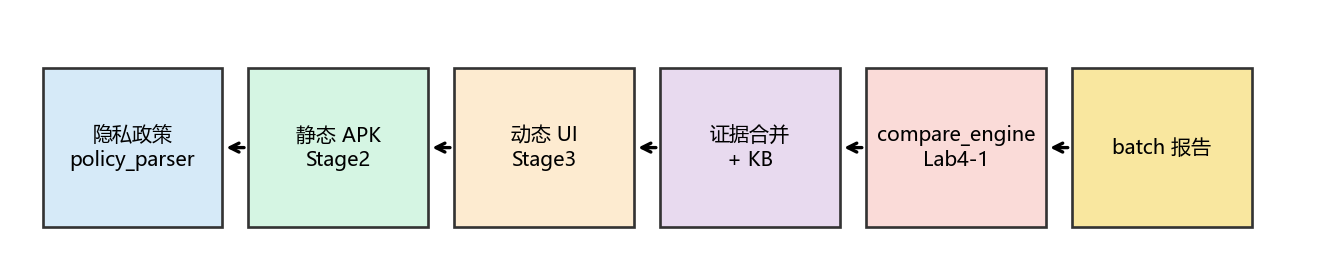
\includegraphics[width=0.98\linewidth]{fig_lab41_pipeline.png}
    \vspace{0.3em}
    \scriptsize
    政策 $\rightarrow$ 静（Stage2）动（Stage3）证据验证 $\rightarrow$ \texttt{lab4\_1\_evidence/\{App\}.json} $\rightarrow$ \texttt{compare\_engine} $\rightarrow$ batch 报告 \\
    政策匹配：先用子串匹配，后用分段聚类和 LLM 增强。\\
    静态: Exodus / Androguard 抽取SDK权限和直接API命中。 \\
    动态: Appium / Frida 运行时使用 hooks 采集运行时证据，并进行别名匹配，包括UI测试和参数截图。 \\
    根据匹配的法律矩阵给出政策文件摘要和置信度，生成证据包。 \\
    使用大语言模型进行比较并生成最终APP报告，为降低幻觉使用JSON格式。 \\
\end{frame}

\begin{frame}
    \frametitle{Lab04-1 核心模块}
    \scriptsize
    \begin{columns}[T]
        \begin{column}{0.5\textwidth}
            \textbf{证据采集与合并}
            \begin{itemize}
                \item \texttt{policy\_parser}：从隐私政策文本匹配个人信息分类，得到 \texttt{declared\_pii}。
                \item \texttt{stage2\_static}：Exodus + Androguard 扫描 APK，生成 \texttt{static\_evidence.json}。
                \item \texttt{stage3\_dynamic}：Appium 导航 + Frida 采集，生成 \texttt{dynamic\_evidence.json}。
                \item \texttt{evidence\_loader}：合并静/动/oldsrc/legacy 等通道，写出 \texttt{lab4\_1\_evidence/\{App\}.json}。
                \item \texttt{privacy\_knowledgebase}：法律矩阵与技术信号推断，补充 \texttt{feasible\_evidence} 与观测类型。
            \end{itemize}
        \end{column}
        \begin{column}{0.46\textwidth}
            \textbf{审计与输出}
            \begin{itemize}
                \item \texttt{compare\_engine}：规则比对声明与观测，输出 \texttt{consistent} 等 verdict。
                \item \texttt{lab4\_1\_report}：汇总 verdicts、\texttt{sources} 与 KB 章节，导出单 App 报告 JSON。
            \end{itemize}
        \end{column}
    \end{columns}
\end{frame}

\begin{frame}
    \frametitle{判定逻辑示意}
    \scriptsize
    \begin{itemize}
        \item \texttt{consistent}：政策声明的类型，在多源证据中可找到支撑。
        \item \texttt{inconsistent\_high\_risk}：证据链观测到某类型，但政策未充分声明（答辩重点）。
        \item \texttt{declared\_not\_observed}：政策声明了，但当前合并证据未观测到。
    \end{itemize}
    \vspace{0.2em}
    \centering
    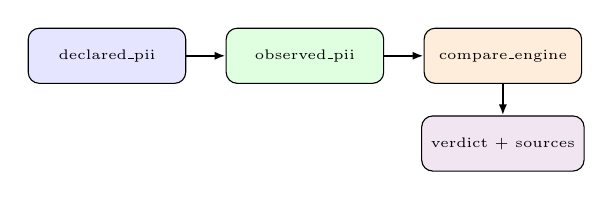
\begin{tikzpicture}[
        node distance=4mm and 5mm,
        box/.style={draw, rounded corners, align=center, minimum width=2.0cm, minimum height=7mm, font=\tiny},
        arr/.style={-{Latex[length=1.4mm]}, thick},
    ]
        \node[box, fill=blue!10] (d) {declared\_pii};
        \node[box, fill=green!12, right=of d] (o) {observed\_pii};
        \node[box, fill=orange!14, right=of o] (c) {compare\_engine};
        \node[box, fill=violet!10, below=of c] (r) {verdict + sources};
        \draw[arr] (d) -- (o);
        \draw[arr] (o) -- (c);
        \draw[arr] (c) -- (r);
    \end{tikzpicture}
\end{frame}

\section{实验设计}

\begin{frame}
    \frametitle{实验环境与样本}
    \small
    \begin{itemize}
        \item \textbf{环境}：Windows + MuMu + Appium \texttt{4723} + Frida（Stage3 辅助，非 Lab4-1 唯一证据源）。
        \item \textbf{10 款 App}：Keep、小红书、支付宝、LOFTER、智联招聘、世纪佳缘、好大夫医生版、东方财富、小荷健康、微信。
        \item \textbf{政策文本}：\texttt{input/pii\_text/\{App\}.txt}
        \item \textbf{证据包}：\texttt{output/lab4\_1\_evidence/\{App\}.json}
        \item \textbf{报告}：\texttt{output/lab4\_1/\{App\}\_lab4\_1\_report.json}
    \end{itemize}
\end{frame}

\begin{frame}
    \frametitle{Stage3 与 UI 适配（证据链一环）}
    \small
    \begin{itemize}
        \item \textbf{世纪佳缘}：底部 Tab 文案为 \texttt{" 我 "}（含空格）。"推荐"界面也存在多处"我"的入口。
        \item \textbf{小荷健康}：「设置」入口仅为齿轮图标且按钮 Label 为空，默认点击右上角最右侧元素（左侧多为扫一扫）。
        \item \textbf{支付宝}：存在「我的…」等入口，需精确匹配文案。
        \item \textbf{东方财富}：不存在"我"的入口，需要点击头像图标，且同时具有用户界面和个人主页。
        \item \textbf{其他 App}：政策路径 token + 精细化别名匹配 + 路径回退兜底。
    \end{itemize}
\end{frame}

\begin{frame}
    \frametitle{Stage3 Corner Cases（真机截图）}
    \small
    以下截图为 \texttt{Lab04-1\_CornorCases} 目录中按 App 整理的 UI 适配难点；每页仅展示一款 App。\\
    \vspace{0.4em}
    \begin{itemize}
        \item \textbf{世纪佳缘}：底部 Tab 为 \texttt{" 我 "}（含空格），推荐页亦有多处「我」入口。
        \item \textbf{东方财富}：无「我」文案入口，需点头像进入个人主页。
        \item \textbf{小荷健康}：「设置」为齿轮图标且 Label 为空，默认点右上角最右侧元素。
    \end{itemize}
\end{frame}

\begin{frame}
    \frametitle{Corner Case：世纪佳缘}
    \scriptsize
    \centering
    Tab 文案 \texttt{" 我 "}（含空格）$\cdot$ 推荐页多处「我」$\cdot$ 路径 token 需精确匹配\\
    \vspace{0.15em}
    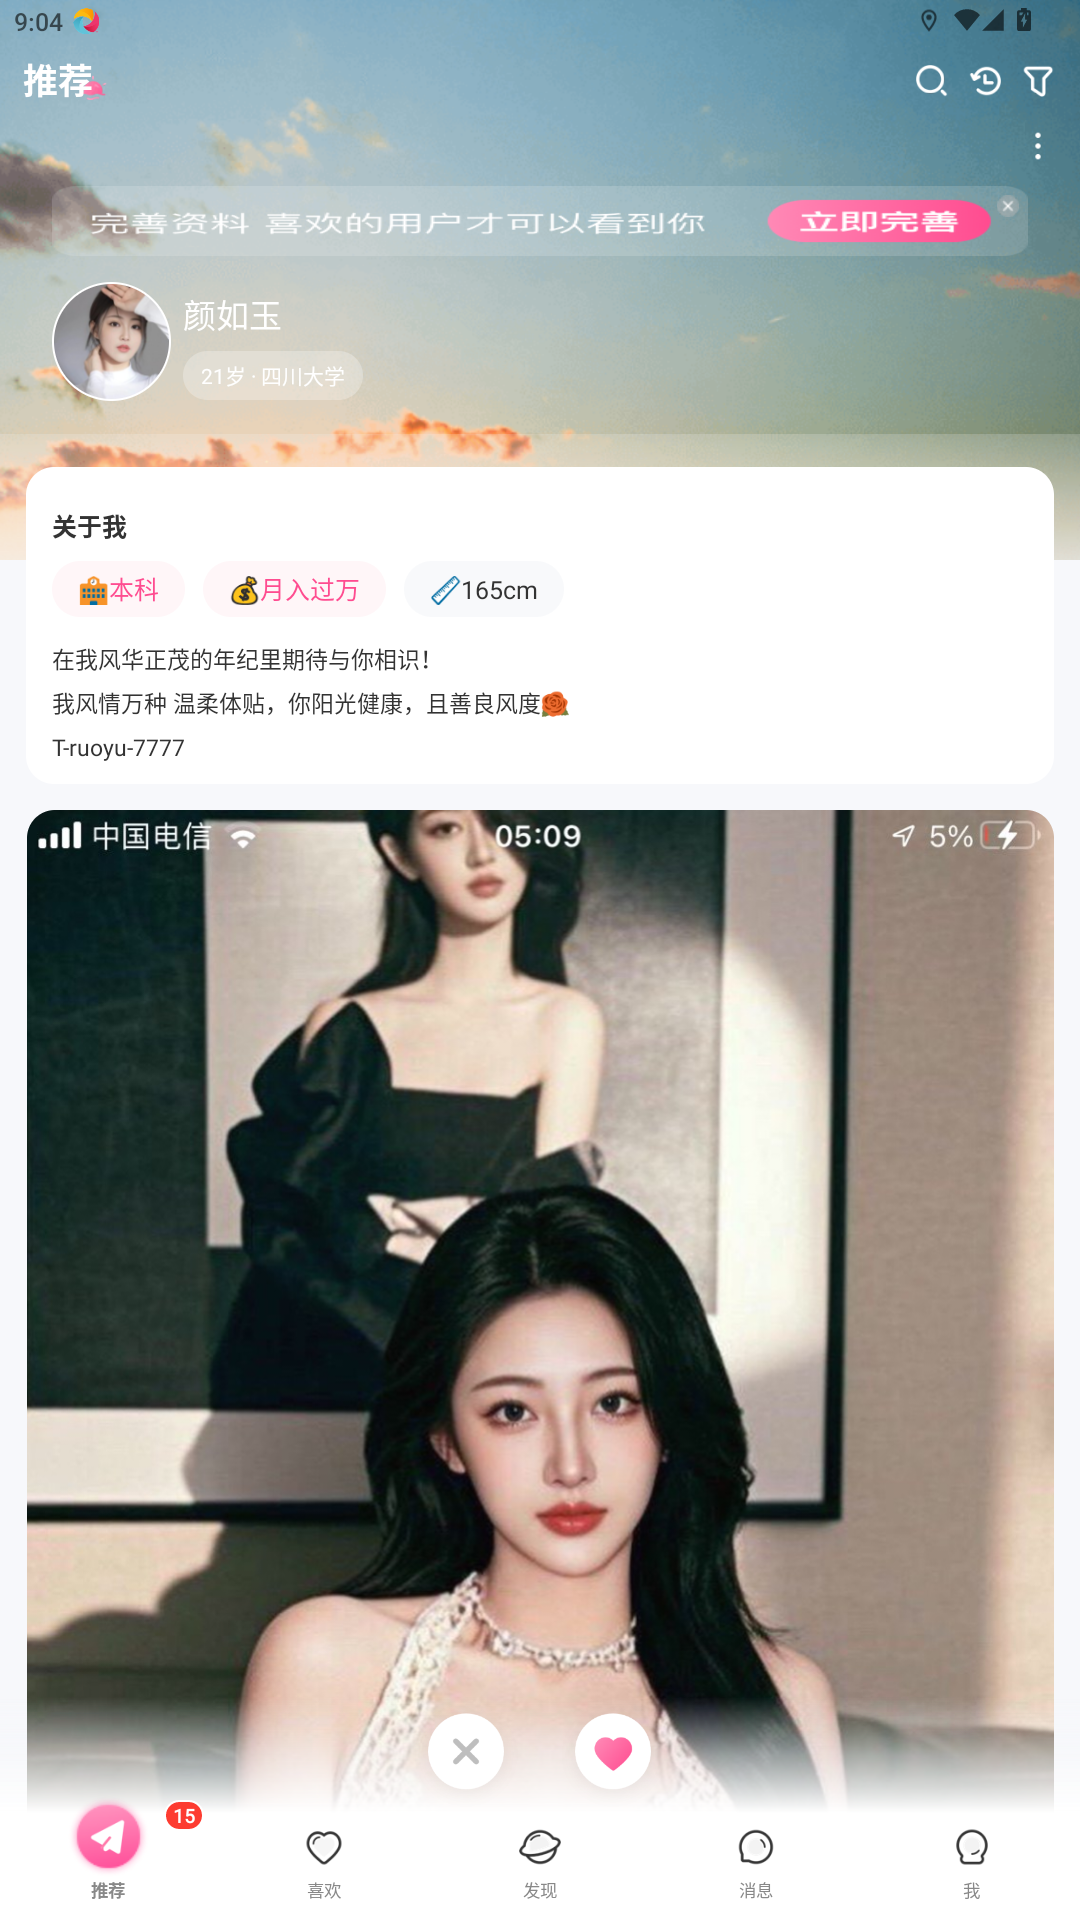
\includegraphics[width=0.31\linewidth]{世纪佳缘_20260524_210447_path2.png}\hfill
    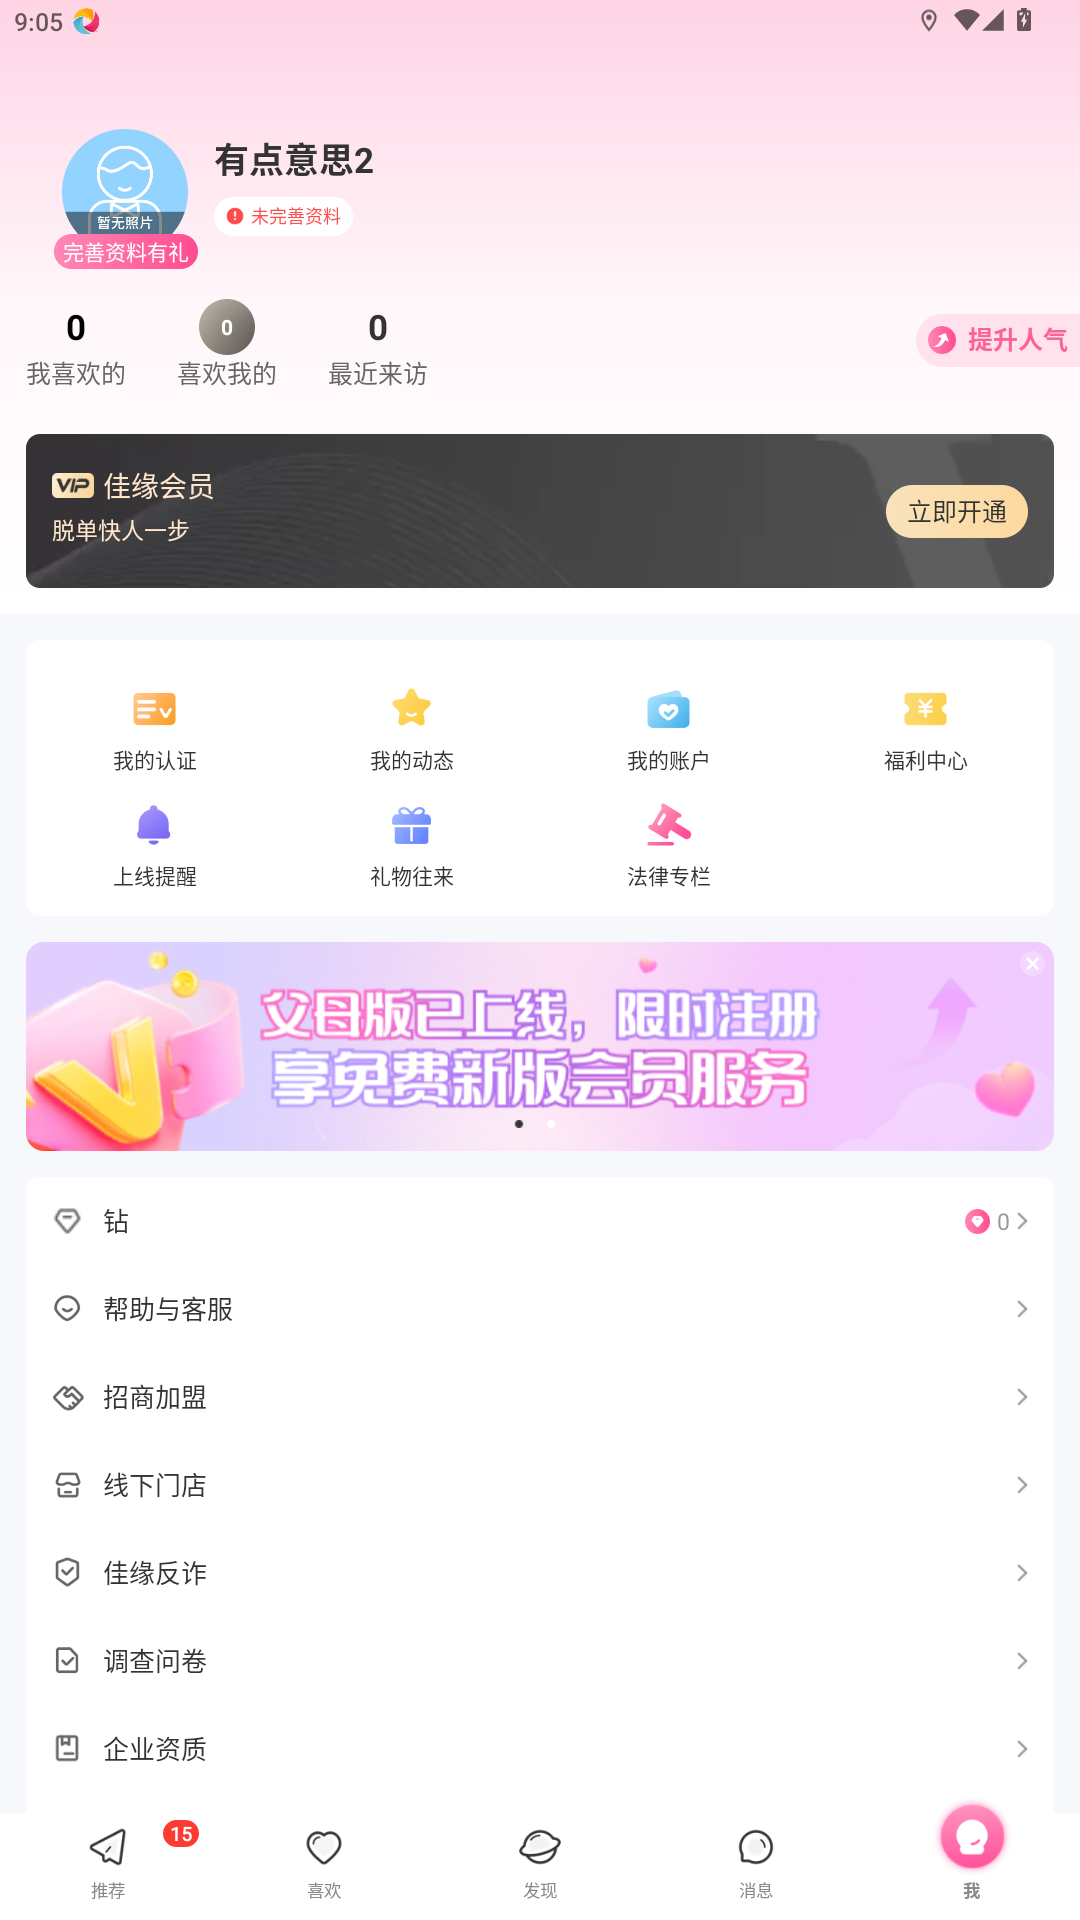
\includegraphics[width=0.31\linewidth]{世纪佳缘_20260524_210504_path2.png}\hfill
    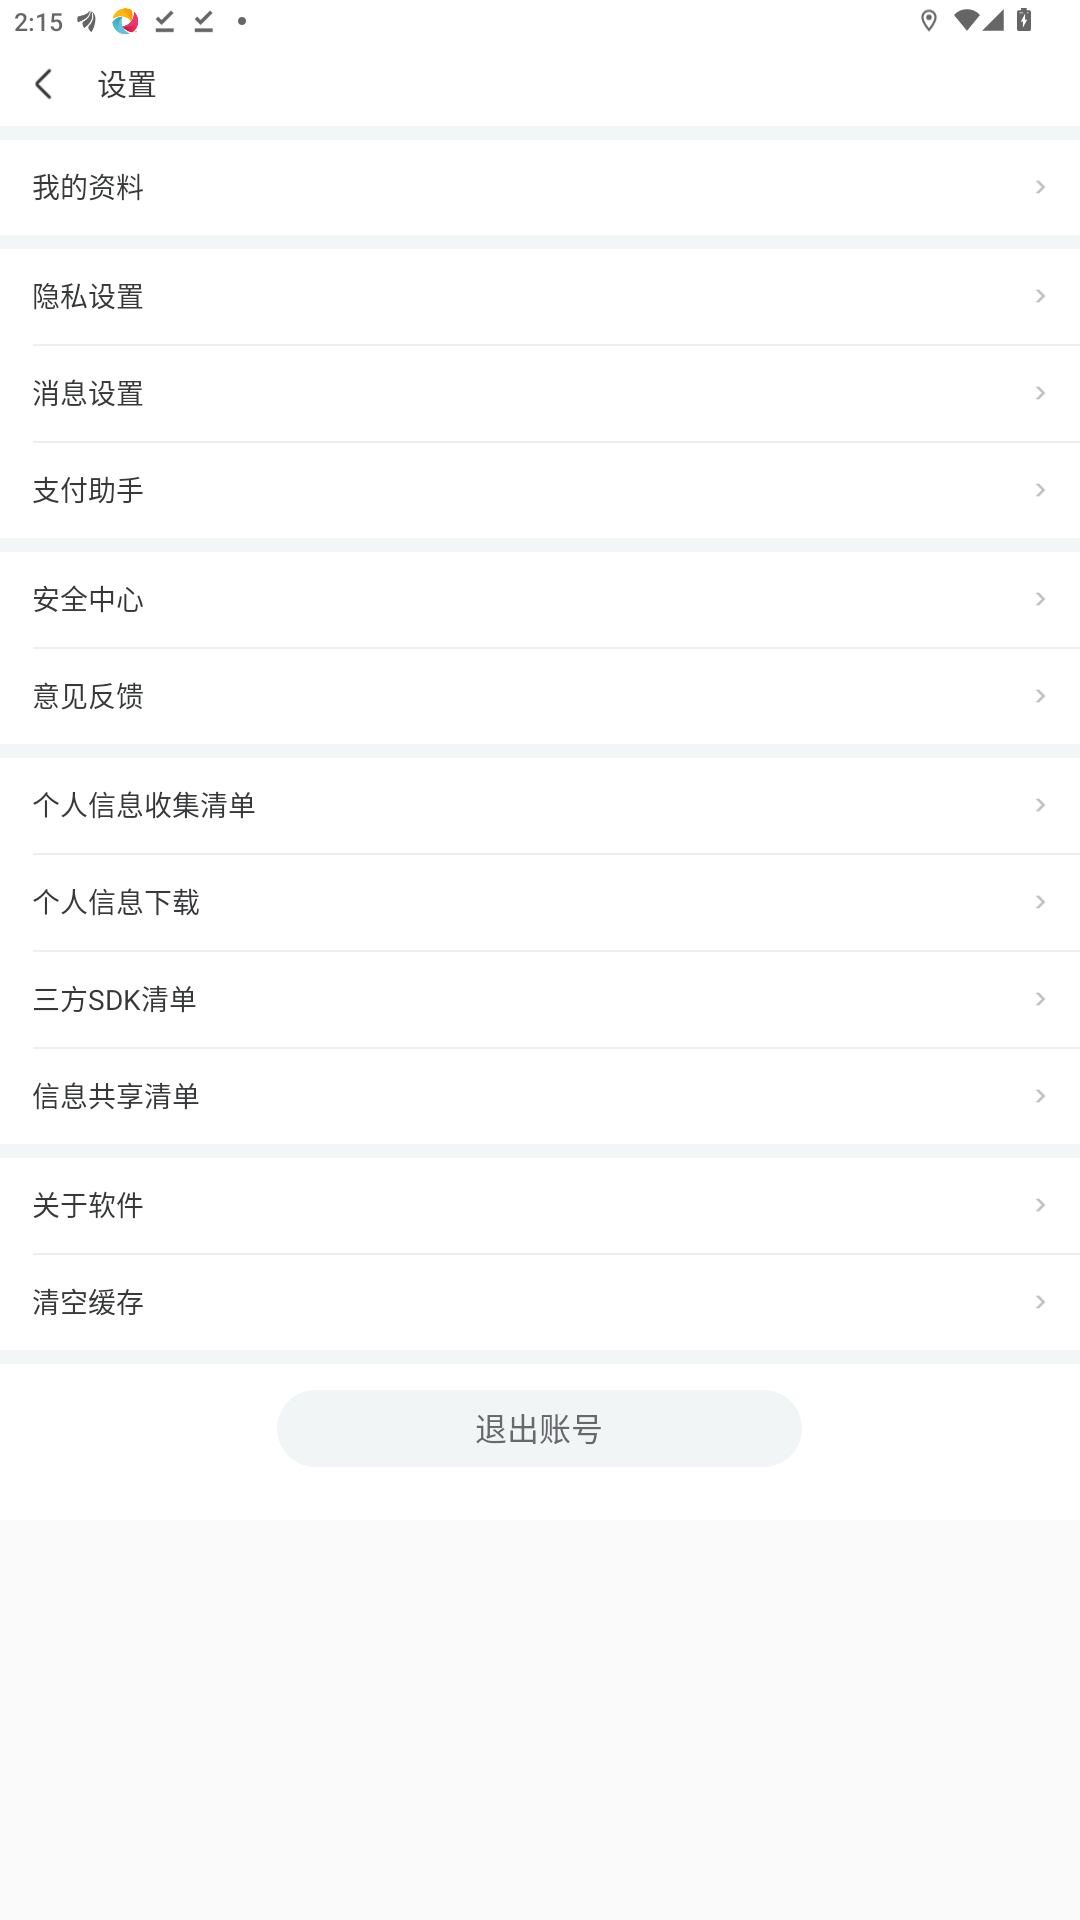
\includegraphics[width=0.31\linewidth]{世纪佳缘_20260525_141550_path1.png}\\[0.25em]
    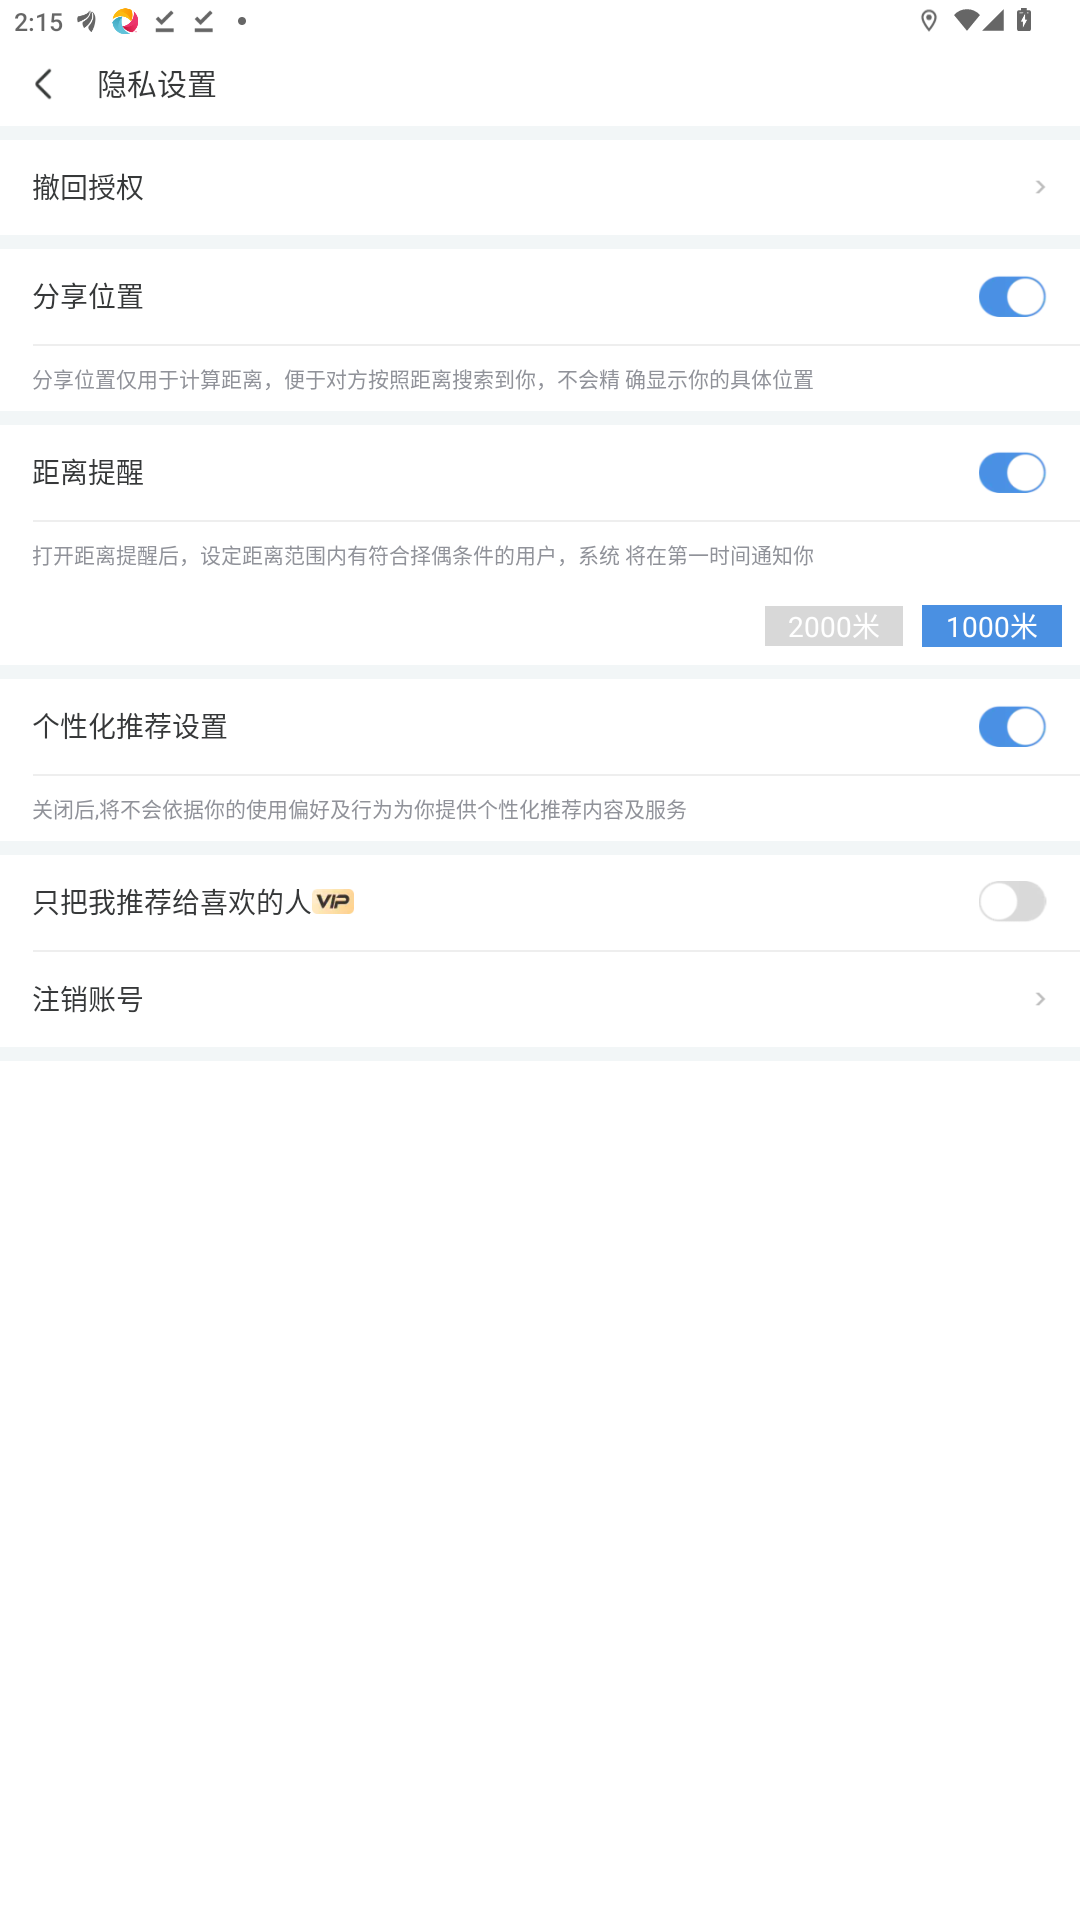
\includegraphics[width=0.38\linewidth]{世纪佳缘_20260525_141552_path1.png}\hfill
    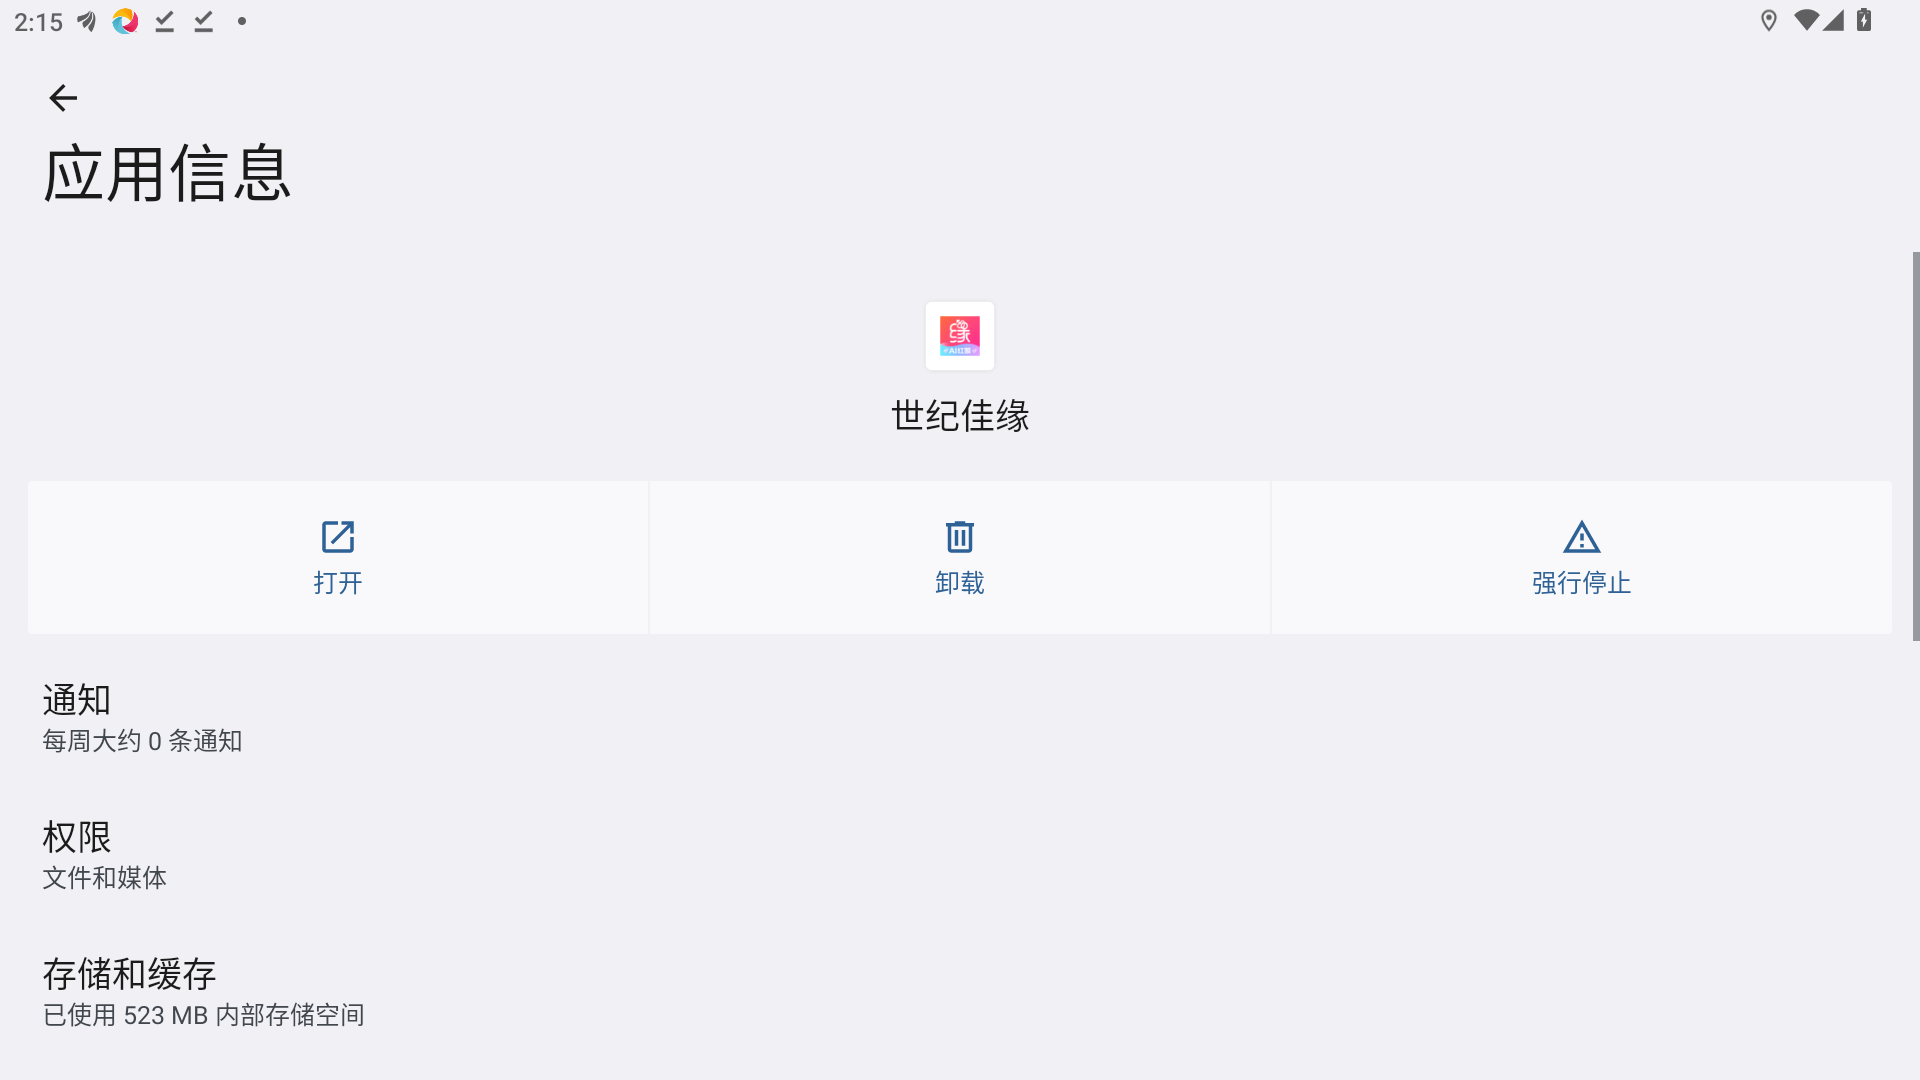
\includegraphics[width=0.38\linewidth]{世纪佳缘_20260525_141553_path1.png}
\end{frame}

\begin{frame}
    \frametitle{Corner Case：东方财富}
    \scriptsize
    \centering
    无「我」入口 $\rightarrow$ 点击头像图标进入个人主页\\
    \vspace{0.3em}
    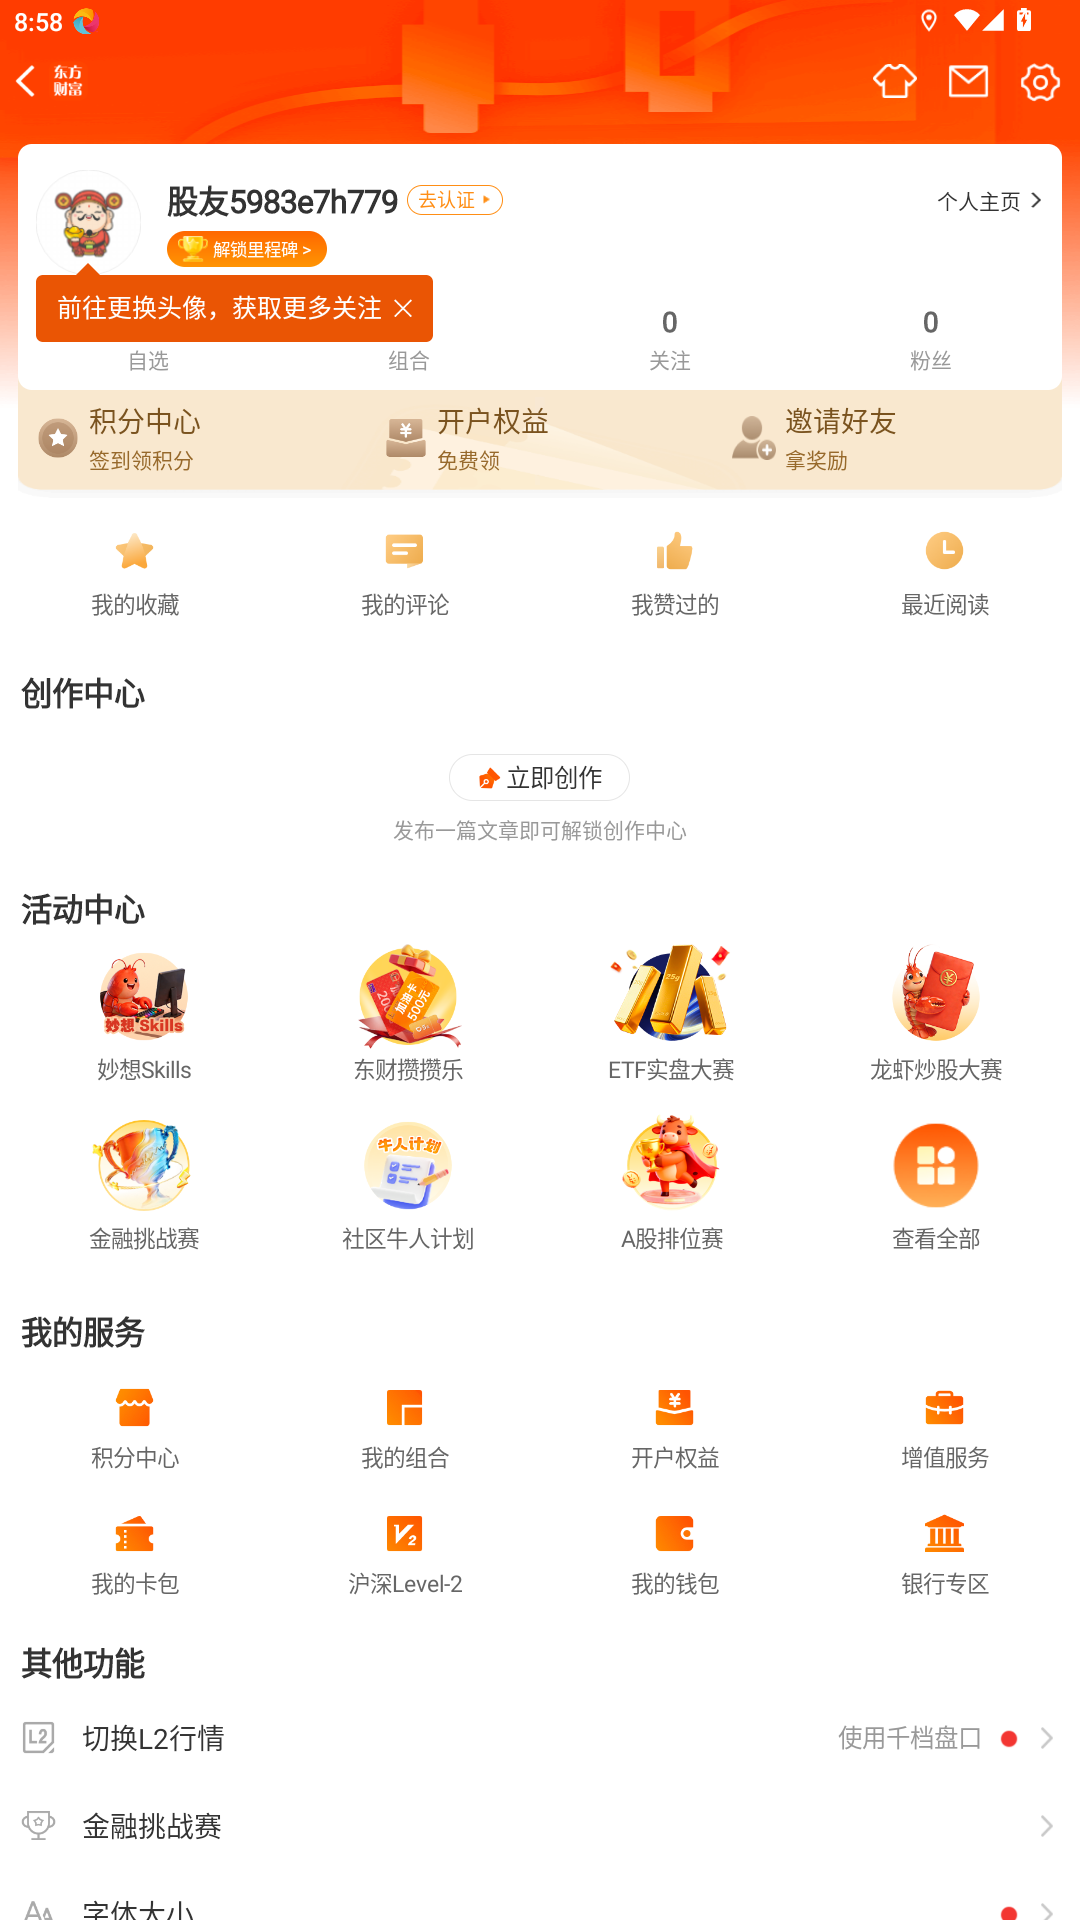
\includegraphics[width=0.46\linewidth]{东方财富_20260524_205836_path2.png}\hfill
    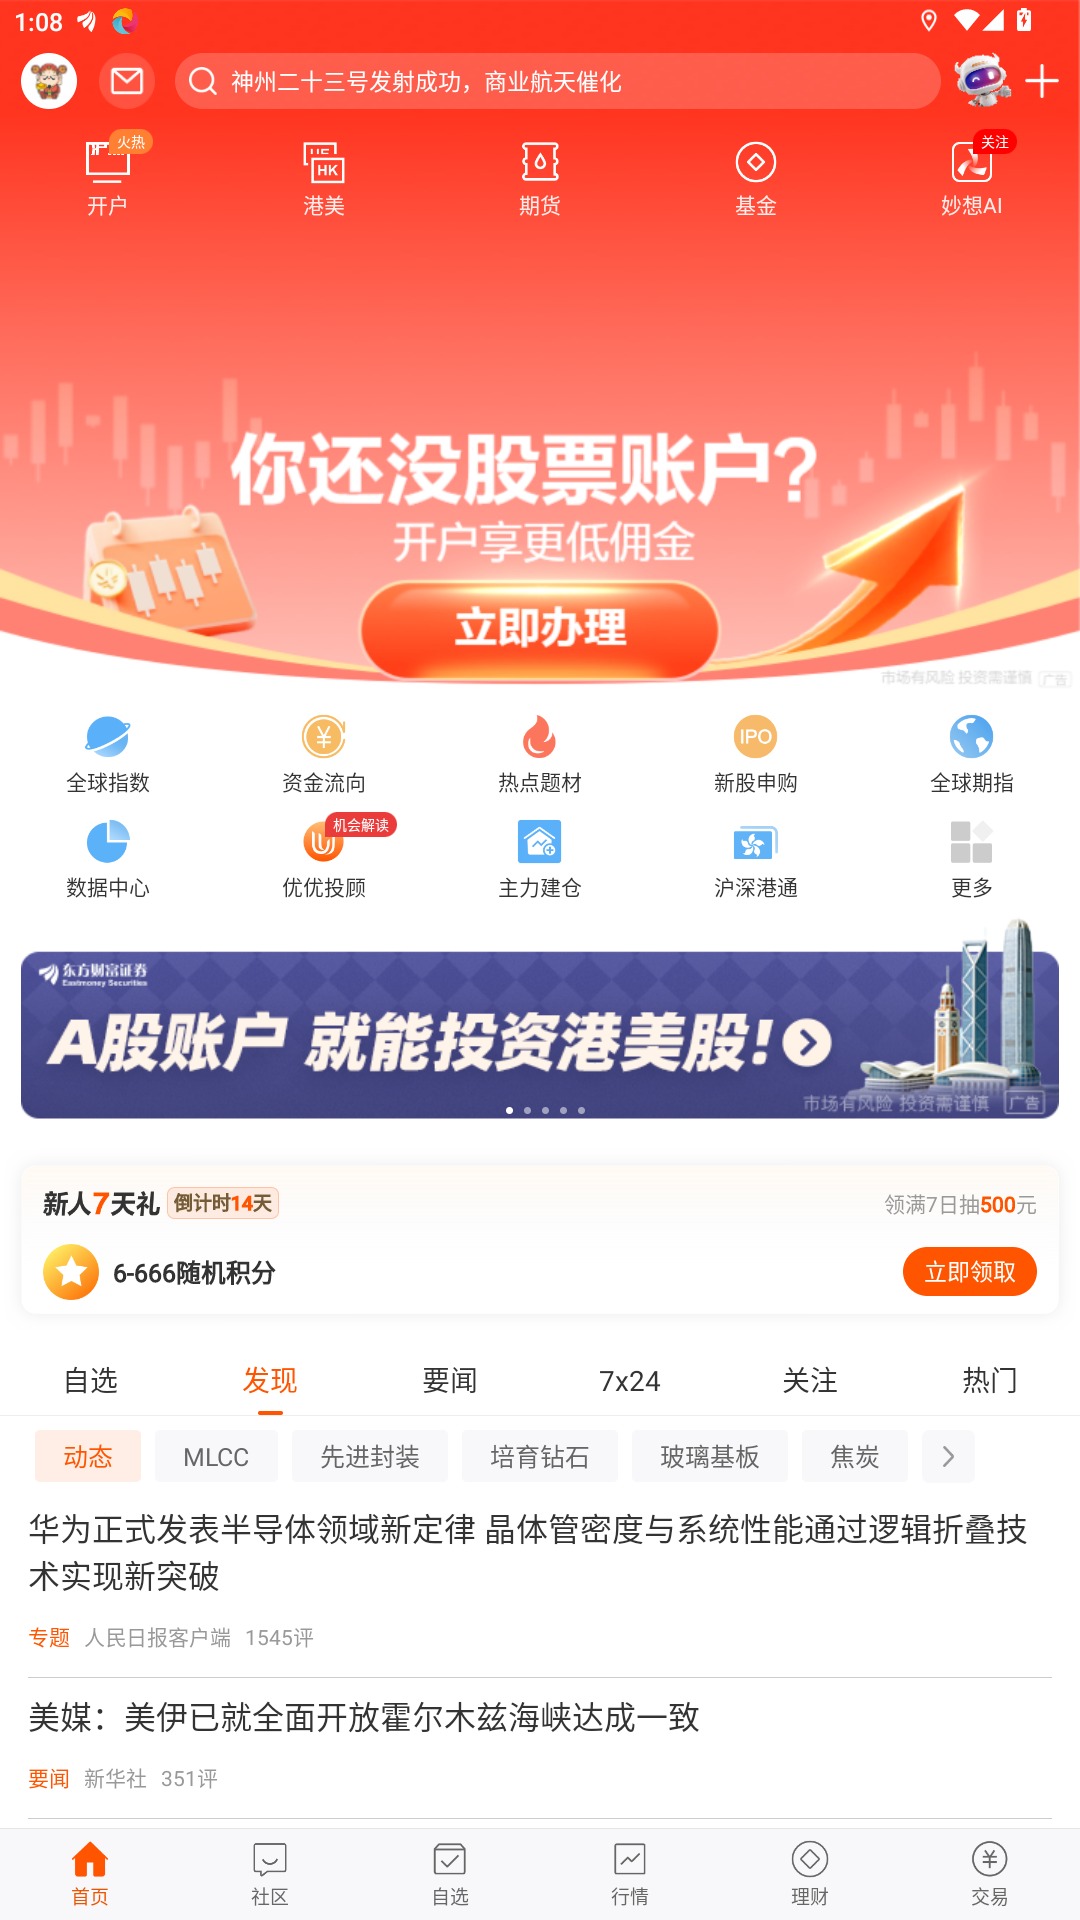
\includegraphics[width=0.46\linewidth]{东方财富_20260525_130802_launch.png}
\end{frame}

\begin{frame}
    \frametitle{Corner Case：小荷健康}
    \scriptsize
    \centering
    「设置」为齿轮图标、无障碍 Label 为空；默认点击右上角最右侧（左侧多为扫一扫）\\
    \vspace{0.3em}
    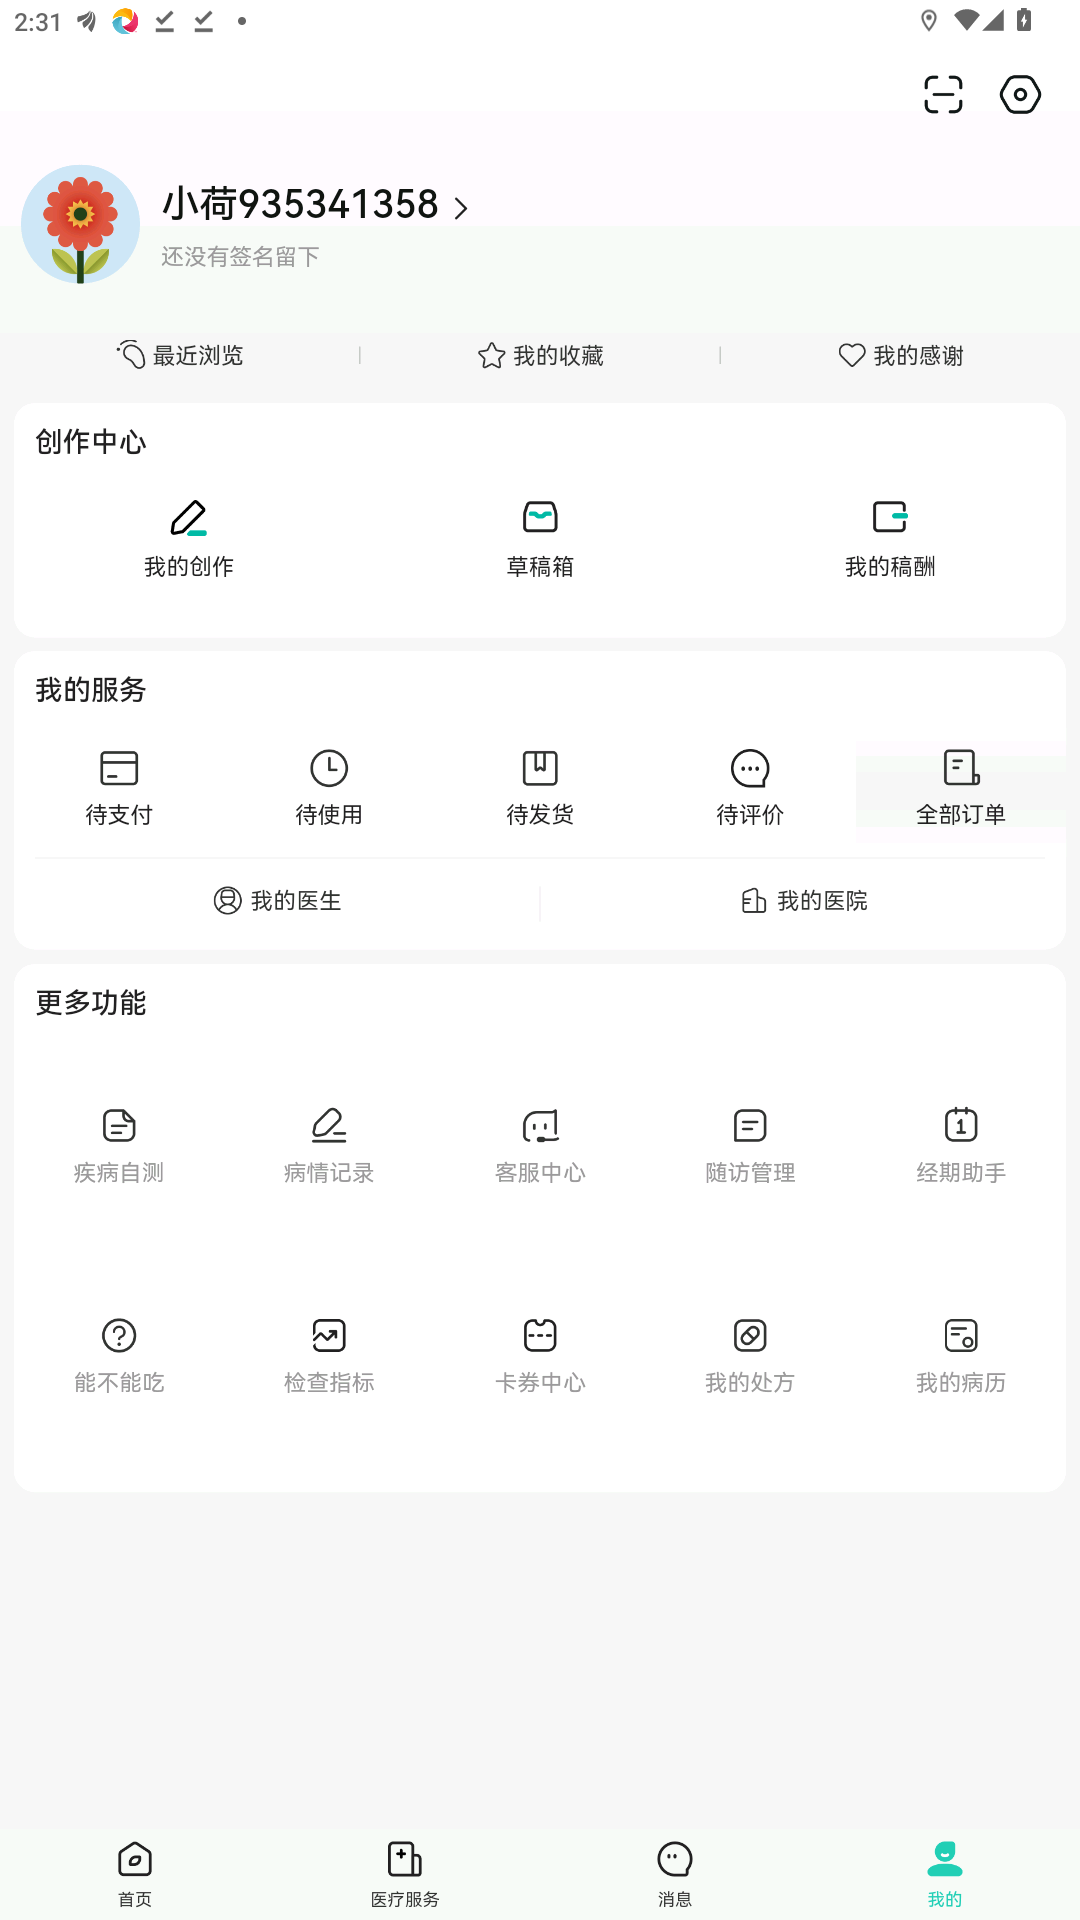
\includegraphics[width=0.55\linewidth]{小荷健康_20260525_143125_path1.png}
\end{frame}


\section{实验结果}

\begin{frame}
    \frametitle{全样本 Verdict 合计}
    \begin{columns}
        \begin{column}{0.42\textwidth}
            \centering
            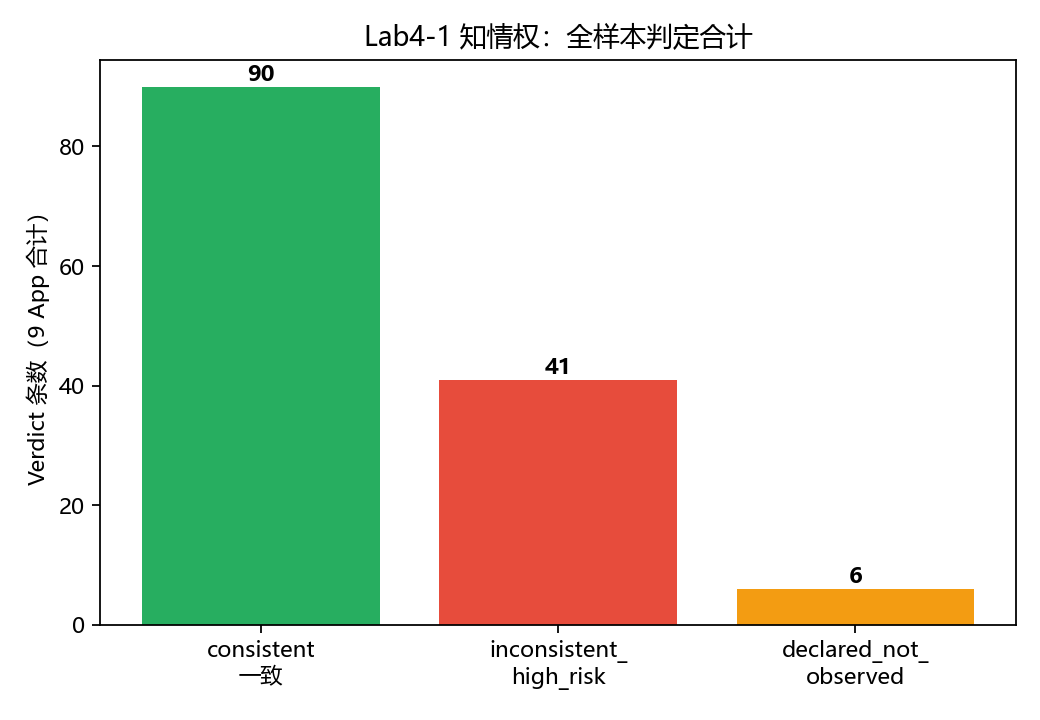
\includegraphics[width=\linewidth]{fig_lab41_verdict_totals.png}
        \end{column}
        \begin{column}{0.54\textwidth}
            \small
            \begin{tabular}{|l|r|}
                \hline
                \textbf{Verdict} & \textbf{条数} \\
                \hline
                consistent & 90 \\
                \hline
                \texttt{inconsistent\_high\_risk} & 41 \\
                \hline
                \texttt{declared\_not\_observed} & 6 \\
                \hline
            \end{tabular}
            \vspace{0.4em}
            \scriptsize
            \begin{itemize}
                \item 一致：声明有、证据也有
                \item 高风险：证据有、声明不足
                \item 未观测：声明有、证据暂无
            \end{itemize}
        \end{column}
    \end{columns}
\end{frame}

\begin{frame}
    \frametitle{declared\_not\_observed 明细（6 条）}
    \scriptsize
    \textbf{含义}：政策 \texttt{declared\_pii} 已声明，当前证据包 \texttt{observed\_pii\_for\_verdict} 未命中；\texttt{risk\_level: medium}。\\
    批次：\texttt{exp\_stage3\_20260525\_lab4\_1}
    \vspace{0.35em}
    \begin{enumerate}
        \item \textbf{好大夫医生版} — \texttt{account\_info}（账号信息）：受限于应用需要资格认证，无法动态验证。
        \item \textbf{世纪佳缘} — \texttt{biometric\_info}（生物识别）：静/动/oldsrc/KB 均未并入。
        \item \textbf{东方财富} — \texttt{log\_info}（日志信息）：声明有，观测列表无此项。
        \item \textbf{世纪佳缘} — \texttt{log\_info}（日志信息）：同上。
        \item \textbf{支付宝} — \texttt{clipboard}（剪贴板）：政策已写，合并证据未列出。
        \item \textbf{智联招聘} — \texttt{clipboard}（剪贴板）：同上。
    \end{enumerate}
    \vspace{0.2em}
    \footnotesize
    世纪佳缘原文："当您开通视频相亲、申请连麦、申请提现时……需要您提供真实身份信息（真实姓名、身份证件号码或人脸信息，根据实际情况可能有所不同）以完成实名认证。" 但实际无法测试人脸信息部分。
\end{frame}

\begin{frame}
    \frametitle{政策声明 vs 合并观测（分 App）}
    \centering
    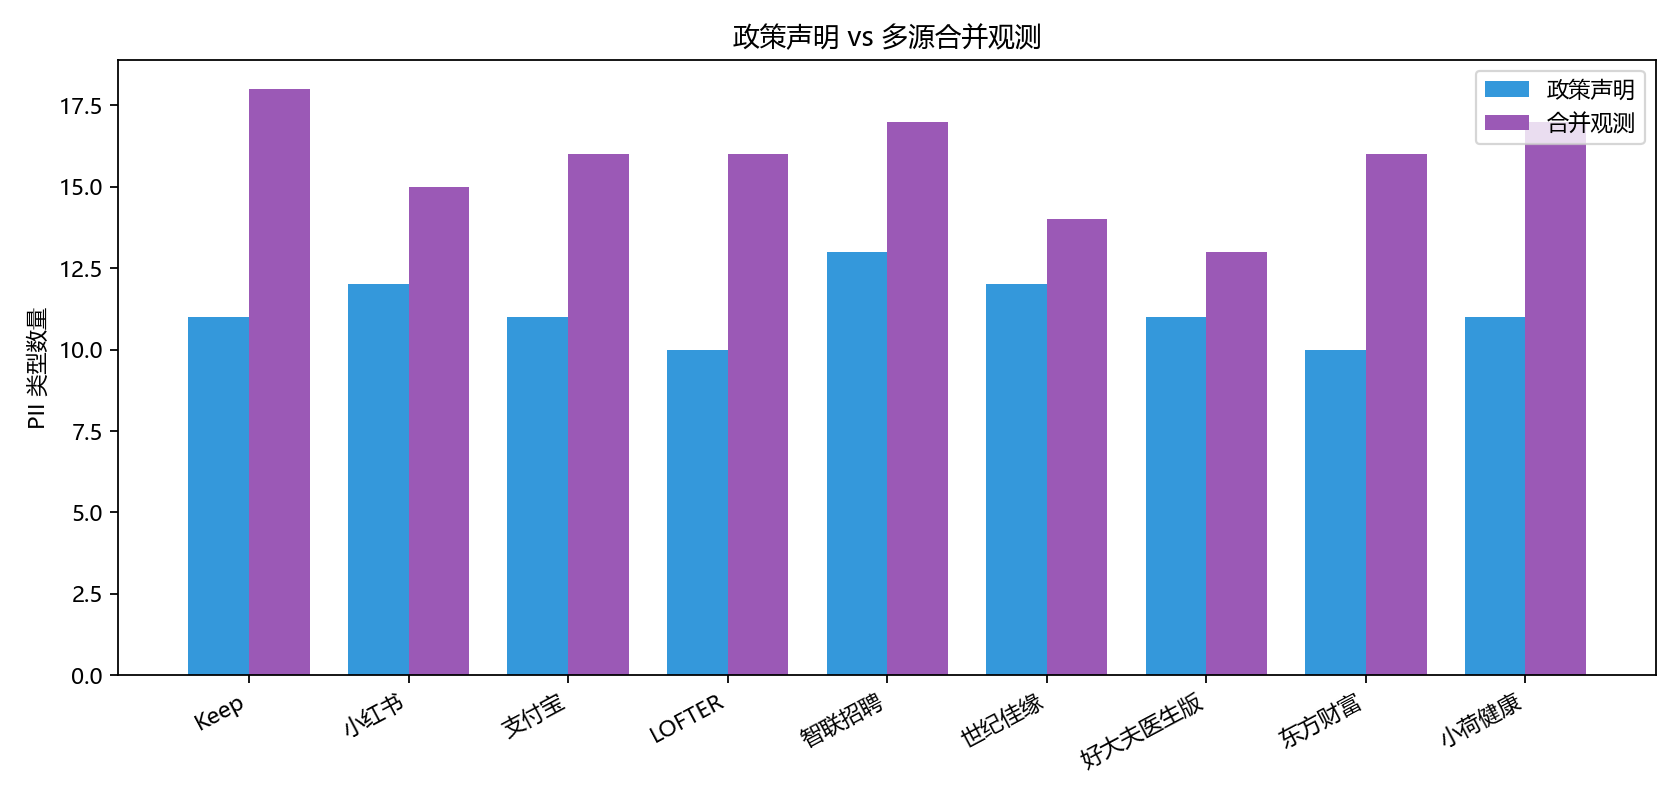
\includegraphics[width=0.95\linewidth]{fig_lab41_declared_observed.png}
    \scriptsize
    多数 App观测类型数 $>$ 声明类型数 $\rightarrow$ 易出现 \texttt{inconsistent\_high\_risk}
\end{frame}

\begin{frame}
    \frametitle{分应用 Verdict 分布}
    \centering
    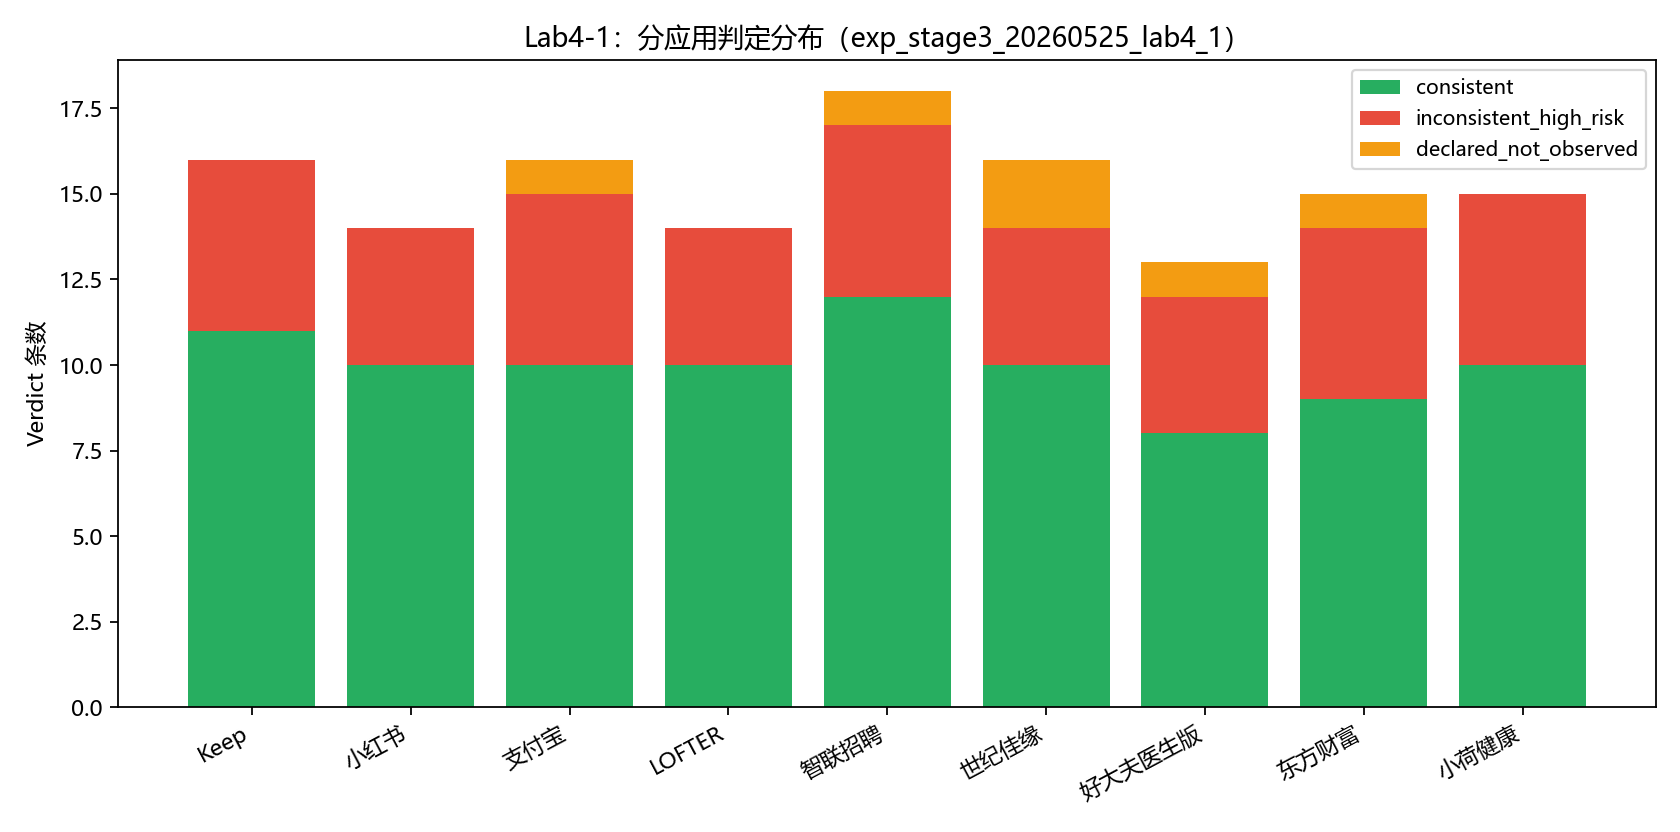
\includegraphics[width=0.95\linewidth]{fig_lab41_verdict_by_app.png}
\end{frame}

\begin{frame}
    \frametitle{分 App 数据表}
    \tiny
    \begin{tabularx}{\textwidth}{|l|r|r|r|r|r|}
        \hline
        \textbf{App} & \textbf{声明} & \textbf{观测} & \textbf{一致} & \textbf{高风险} & \textbf{未观测} \\
        \hline
        Keep & 11 & 18 & 11 & 5 & 0 \\
        \hline
        小红书 & 12 & 15 & 10 & 4 & 1 \\
        \hline
        支付宝 & 11 & 16 & 10 & 5 & 1 \\
        \hline
        LOFTER & 10 & 16 & 10 & 4 & 2 \\
        \hline
        智联招聘 & 13 & 17 & 12 & 5 & 0 \\
        \hline
        世纪佳缘 & 12 & 14 & 10 & 4 & 2 \\
        \hline
        好大夫医生版 & 11 & 13 & 8 & 4 & 1 \\
        \hline
        东方财富 & 10 & 16 & 9 & 5 & 2 \\
        \hline
        小荷健康 & 11 & 17 & 10 & 5 & 0 \\
        \hline
    \end{tabularx}
    \vspace{0.25em}
    \scriptsize
\end{frame}

% --- 分 App 声明 / 观测 / 高风险 / 未观测（批次 exp\_stage3\_20260525\_lab4\_1）---

\begin{frame}
    \frametitle{具体隐私内容（Keep）}
    \apppiidetail{11}{账号, AndroidID, 身份, IMEI, IP, 位置, 日志, 未成年人, 权限, 手机号, 画像}{18}{账号, AndroidID, 生物识别, 剪贴板, 通讯录, 身份, IMEI, IP, 位置, 日志, MAC, 未成年人, 权限, 手机号, 画像, 权利, SDK, 安全}
    \textbf{高风险（5）}：剪贴板, 通讯录, 权利, SDK, 安全\\
    \textbf{未观测（0）}：无
\end{frame}

\begin{frame}
    \frametitle{具体隐私内容（小红书）}
    \apppiidetail{12}{账号, AndroidID, 通讯录, 身份, IMEI, IP, 位置, 日志, MAC, 未成年人, 权限, 手机号}{15}{账号, AndroidID, 生物识别, 通讯录, IMEI, IP, 位置, MAC, 未成年人, 权限, 手机号, 画像, 权利, SDK, 安全}
    \textbf{高风险（4）}：画像, 权利, SDK, 安全\\
    \textbf{未观测（0）}：无
\end{frame}

\begin{frame}
    \frametitle{具体隐私内容（支付宝）}
    \apppiidetail{11}{账号, AndroidID, 生物识别, 剪贴板, 通讯录, 身份, IMEI, IP, 位置, MAC, 手机号}{16}{账号, AndroidID, 生物识别, 通讯录, 身份, IMEI, IP, 位置, MAC, 未成年人, 权限, 手机号, 画像, 权利, SDK, 安全}
    \textbf{高风险（5）}：未成年人, 权限, 权利, SDK, 安全\\
    \textbf{未观测（1）}：剪贴板
\end{frame}

\begin{frame}
    \frametitle{具体隐私内容（LOFTER）}
    \apppiidetail{10}{账号, AndroidID, 身份, IMEI, IP, 位置, 日志, MAC, 权限, 手机号}{16}{账号, AndroidID, 生物识别, 通讯录, 身份, IMEI, IP, 位置, 日志, MAC, 权限, 手机号, 画像, 权利, SDK, 安全}
    \textbf{高风险（4）}：通讯录, 权利, SDK, 安全\\
    \textbf{未观测（0）}：无
\end{frame}

\begin{frame}
    \frametitle{具体隐私内容（智联招聘）}
    \apppiidetail{13}{账号, AndroidID, 生物识别, 剪贴板, 通讯录, 身份, IMEI, IP, 位置, 日志, MAC, 权限, 手机号}{17}{账号, AndroidID, 生物识别, 通讯录, 身份, IMEI, IP, 位置, 日志, MAC, 未成年人, 权限, 手机号, 画像, 权利, SDK, 安全}
    \textbf{高风险（5）}：未成年人, 画像, 权利, SDK, 安全\\
    \textbf{未观测（1）}：剪贴板
\end{frame}

\begin{frame}
    \frametitle{具体隐私内容（世纪佳缘）}
    \apppiidetail{12}{账号, AndroidID, 生物识别, 通讯录, 身份, IMEI, IP, 位置, 日志, MAC, 权限, 手机号}{14}{账号, AndroidID, 通讯录, 身份, IMEI, IP, 位置, MAC, 权限, 手机号, 画像, 权利, SDK, 安全}
    \textbf{高风险（4）}：画像, 权利, SDK, 安全\\
    \textbf{未观测（2）}：生物识别, 日志
\end{frame}

\begin{frame}
    \frametitle{具体隐私内容（好大夫医生版）}
    \apppiidetail{11}{账号, AndroidID, 生物识别, 身份, IMEI, IP, 位置, 日志, MAC, 权限, 手机号}{13}{AndroidID, 生物识别, 通讯录, IMEI, IP, 位置, MAC, 未成年人, 权限, 手机号, 画像, 权利, 安全}
    \textbf{高风险（4）}：通讯录, 未成年人, 权利, 安全\\
    \textbf{未观测（1）}：账号
\end{frame}

\begin{frame}
    \frametitle{具体隐私内容（东方财富）}
    \apppiidetail{10}{账号, AndroidID, 身份, IMEI, IP, 位置, 日志, MAC, 权限, 手机号}{16}{账号, AndroidID, 生物识别, 通讯录, 身份, IMEI, IP, 位置, MAC, 未成年人, 权限, 手机号, 画像, 权利, SDK, 安全}
    \textbf{高风险（5）}：未成年人, 画像, 权利, SDK, 安全\\
    \textbf{未观测（1）}：日志
\end{frame}

\begin{frame}
    \frametitle{具体隐私内容（小荷健康）}
    \apppiidetail{11}{账号, AndroidID, 身份, IMEI, IP, 位置, 日志, MAC, 未成年人, 权限, 手机号}{17}{账号, AndroidID, 生物识别, 剪贴板, 通讯录, 身份, IMEI, IP, 位置, MAC, 未成年人, 权限, 手机号, 画像, 权利, SDK, 安全}
    \textbf{高风险（5）}：剪贴板, 通讯录, 画像, 权利, 安全\\
    \textbf{未观测（0）}：无
\end{frame}

\begin{frame}
    \frametitle{9 App 类型并集与交集}
    \tiny
    \begin{tabularx}{\textwidth}{|l|X|X|}
        \hline
        & \textbf{并集（至少 1 款 App 出现）} & \textbf{交集（9 款 App 均有）} \\
        \hline
        声明 & 账号, AndroidID, 生物识别, 剪贴板, 通讯录, 身份, IMEI, IP, 位置, 日志, MAC, 未成年人, 权限, 手机号, 画像（15 类） & 账号, AndroidID, 身份, IMEI, IP, 位置, 手机号（7 类） \\
        \hline
        观测 & 上列 + 权利, SDK, 安全（18 类） & AndroidID, 通讯录, IMEI, IP, 位置, MAC, 权限, 手机号, 画像, 权利, 安全（11 类） \\
        \hline
        高风险 & 剪贴板, 通讯录, 未成年人, 权限, 画像, 权利, SDK, 安全（8 类） & 权利, 安全（2 类） \\
        \hline
        未观测 & 账号, 生物识别, 剪贴板, 日志（4 类） & 无 \\
        \hline
    \end{tabularx}
    \vspace{0.3em}
    \scriptsize
    高风险 = \texttt{inconsistent\_high\_risk}；未观测 = \texttt{declared\_not\_observed}。\\
    并集观测 18 类中，仅 Keep/小荷等在\textbf{声明}侧含剪贴板；9 款交集声明仅 7 类，反映政策表述差异。
\end{frame}

\section{总结与展望}

\begin{frame}
    \frametitle{阶段性结论}
    \small
    \begin{itemize}
        \item 完成 \textbf{9 App Lab4-1 知情权}批量审计，工程流水线稳定（9/9）。
        \item 规则引擎产出结构化判定（一致 90 + 高风险 41 + 未观测 6），可溯源、可复核。
        \item 主要发现：\textbf{41 条高风险不一致}，反映「观测类型多于政策声明」的普遍模式。
        \item 汇报边界：已说明证据多源性与 Frida 运行时局限；Lab4-2/3 留作后续工作。
    \end{itemize}
\end{frame}

\begin{frame}
    \frametitle{判定伦理与监管话语：「隐瞒采集」为何更重？}
    \small
    \begin{block}{核心判断}
        「未声明但观测到」优先于「声明但未观测到」——在\textbf{监管执法叙事}中较普遍，但\textbf{不是}法条中的固定数学公式。
    \end{block}
    \vspace{0.2em}
    本系统 \texttt{inconsistent\_high\_risk} / \texttt{declared\_not\_observed} 的权重设计，对齐的是\textbf{执法与测评实践中的侧重点}，而非声称「法律只惩罚前者」。
\end{frame}

\begin{frame}
    \frametitle{中国近年 App 个人信息治理：高频执法主题}
    \small
    通报、专项整治与典型违法案例中，常见表述包括：
    \begin{itemize}
        \item \textbf{未告知、未明示}处理目的、方式、范围；
        \item \textbf{实际收集与告知不一致}、默认收集、强制索权；
        \item \textbf{SDK 违规}、后台自启动、\textbf{超范围收集}。
    \end{itemize}
    \vspace{0.3em}
    监管与公众直觉里，「\textbf{没告诉用户就采了}」往往比「\textbf{政策写了很多但本次测评没抓到}」更容易被定性为明确违法或高风险，也更容易进入通报名单。
\end{frame}

\begin{frame}
    \frametitle{告知通胀：另一类问题，但落地路径不同}
    \small
    「政策过宽、笼统、堆砌」（\textbf{告知通胀}）同样会被批评，涉嫌违反\textbf{明确、合理、必要}及误导用户。
    \begin{itemize}
        \item 处罚落地往往需结合：\textbf{是否真采集}、\textbf{最小必要}、\textbf{同意是否有效}；
        \item 自动化测评中 \texttt{declared\_not\_observed} $\neq$ 监管已认定「恶意夸大」，更多表示\textbf{待核查}或\textbf{测试局限}；
        \item 本系统 KB 对「声明但未观测」的放宽，体现的是\textbf{证据不足时克制判高风险}，而非认可笼统告知。
    \end{itemize}
\end{frame}

\begin{frame}
    \frametitle{国际对照（GDPR）与本系统定位}
    \small
    \begin{itemize}
        \item GDPR：\textbf{缺乏透明度}与\textbf{缺乏合法依据}均可严重违规；对外执法叙事中，\emph{secret processing}（用户不知情的处理）冲击力通常大于冗长、模糊的隐私政策。
        \item 后者多走 \textbf{transparency + fairness} 路径，需结合实务评估，通常不会仅凭「本次未观测到」即定论。
        \item \textbf{本 Lab4-1}：规则 + 证据驱动的声明—观测对齐；更敏感于 \texttt{not\_declared \& observed}，对 \texttt{declared \& not\_observed} 在 KB 下保留复核空间——与当前主流\textbf{测评/执法权重}同向，但局限于声明膨胀、观测假阳性等。
    \end{itemize}
\end{frame}

\begin{frame}
    \frametitle{市场阶段：规则已有，标准仍在细化}
    \scriptsize
    \begin{tabularx}{\textwidth}{|l|X|c|}
        \hline
        \textbf{阶段特征} & \textbf{说明} & \textbf{是否符合} \\
        \hline
        开放、监管缺位 & PIPL、国标、App 备案、SDK 规定、专项整治、应用商店规则等已建立 & 基本\textbf{已过} \\
        \hline
        规范建立、健康发展（过渡） & 类型划分与「告知—行为」对齐标准、自动化口径仍在演进；执法\textbf{有节奏、有重点}（先打未告知、超范围、SDK 等硬伤） & \textbf{最符合} \\
        \hline
        完全成熟、可机械打分 & 场景差异大；政策—代码无全国统一自动判据；「测不全」与「真未采」难区分 & \textbf{尚不符合} \\
        \hline
    \end{tabularx}
    \vspace{0.4em}
    \small
    「更重隐瞒采集」是\textbf{过渡型市场}中常见的监管伦理：方向已明，执行上先抓危害感知强、证据较易认定的问题；对「写得太多/测不到」侧重\textbf{改进告知 + 抽查核实}，而非一律按「窃取」论处。
\end{frame}

\begin{frame}
    \frametitle{展望与后续工作}
    \small
    \begin{itemize}
        \item \textbf{局限补强}：关注告知通胀（宽泛声明降低 \texttt{not\_declared} 命中率）；区分 \texttt{inconsistent\_high\_risk}（技术）与 \texttt{kb\_inferred\_undeclared}（仅 KB）。
        \item \textbf{工程延伸}：Lab4-2 同意、Lab4-3 访问/更正/删除；可选增加「过度声明/模糊用语」指标，与知情权审计互补。
        \item \textbf{研究定位}：本系统宜定位为\textbf{过渡市场中的告知—行为对齐审计工具}，而非全面法律合规的终局评分器。
    \end{itemize}
\end{frame}

\begin{frame}
    \begin{center}
        {\Huge 感谢聆听！}\\[0.8em]
        {\large Q \& A}
    \end{center}
\end{frame}

\end{document}
